\documentclass[table]{beamer}
%\usepackage[table]{xcolor}
\usepackage{amsmath, amsfonts, epsfig, xspace}
\usepackage[utf8]{inputenc}
\usepackage{algorithm,algorithmic}
\usepackage[normal,tight,center]{subfigure}
\setlength{\subfigcapskip}{-.5em}
\usepackage{beamerthemesplit}
% \usetheme{lankton-keynote}
\setbeamertemplate{headline}{} %Hide section stuff
\usepackage{natbib} %schönere Zitate
\usepackage{color}
\definecolor{OliveGreen}{RGB}{0,155,85}

\author{Jonathan Oberländer}

\title[Automatic Detection of LQ Violations\hspace{8em}\insertframenumber]{Automatic Detection of Linguistic Quality Violations} %\insertframenumber/\inserttotalframenumber

\date{}

\institute{Bachelor Thesis Defense\\Universität des Saarlandes\\21.08.2014}

\begin{document}

\maketitle

\section{Automatic Summarization}

\begin{frame}
  \frametitle{Automatic Summarization}
  \quad \quad 
\includegraphics[scale=0.1]{pics/documents.png} 
\includegraphics[scale=1]{pics/arrowlr.png} 
\includegraphics[scale=0.1]{pics/document.png}
\end{frame}

\begin{frame}
  \frametitle{Automatic Summarization}
  %types
  \begin{itemize}
    \item \textbf{Single-Document:} One document
    \item \textbf{Multi-Document:} Multiple documents on the same topic
  \end{itemize}
  \pause
  \begin{itemize}
    \item \textbf{Abstractive:} Internal semantic representation + generation
    \item \textbf{Extractive:} New summary from source sentences
  \end{itemize}
  \pause
  \vspace{1cm}

  \quad \quad \quad \begin{tabular}{r|c|c|}
    & Single-document & Multi-document\\
    \hline
    Abstractive & \cellcolor{red!25} & \cellcolor{red!25}\\
    \hline
    Extractive & \cellcolor{red!25} & \cellcolor{green!25}\\
    \hline
  \end{tabular}
  %…which hopefully produces coherent, grammatical sentences.
\end{frame}

\begin{frame}
  \frametitle{Linguistic Quality Violations}
  \textbf{Summarization systems \only<2->{\textcolor{red}{don't}}\only<1>{should} produce coherent and grammatical output.}
  \pause

  \textbf{Why?}
  \begin{itemize}
    \item It's hard.\pause
    \item Evaluation: content, information density
  \end{itemize}
  \vspace{1cm}
  \pause
  $\Rightarrow$ LQVCorpus \citep{friedrichlqvsumm}

  %doesn't always work. Why?

\end{frame}

\begin{frame}
  \frametitle{LQVCorpus \citep{friedrichlqvsumm}}
  %eckdaten, was wurde annotiert
  Annotated results of TAC 2011 Guided Summarization task \citep{owczarzak2011overview}
\pause
  \begin{itemize}
    \item Entity level:
    \begin{itemize}
      \item FM-EXPL, SM+EXPL%first mention without explanation%subsequent mention with explanation
      \item DNP-REF, INP+REF%definite noun phrase without reference to previous mention%indefinite noun phrase with reference to previous mention
      \item PRN-ANT, PRN+MISLA%pronoun with missing antecedent%pronoun with misleading antecedent
      \item ACR-EXPL%acronyms without explanations
    \end{itemize}\pause
    \item Clause level:
    \begin{itemize}
      \item \textbf{incomplete sentence (INCOMPLSN)}
      \item \textbf{inclusion of datelines (INCLDATE)}
      \item \textbf{other ungrammatical form (OTHRUNGR)}
      \item no semantic relatedness (NOSEMREL)
      \item \textbf{redundant information (REDUNINF)}
      \item no discourse relation (NODISREL)
    \end{itemize}
  \end{itemize}
\end{frame}

\begin{frame}
  \frametitle{Detecting Ungrammaticality (OTHRUNGR)}
  %Many subtypes of ungrammaticality
  % \begin{itemize}
  %   \item Corpus study: actually many different types of violations
  % \end{itemize}
  \begin{center}
    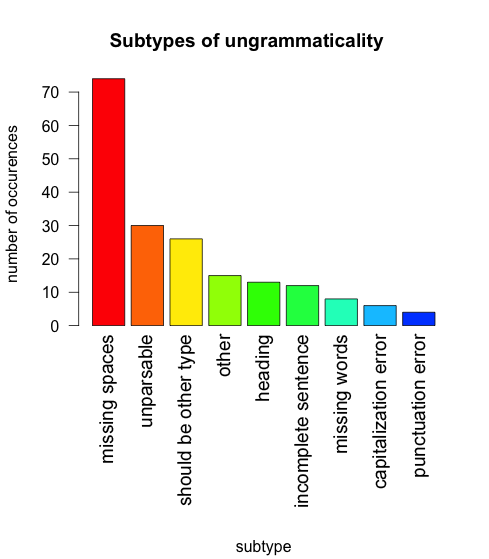
\includegraphics[scale=0.4]{subtypes_dev2.png}
  \end{center}
\end{frame}

\begin{frame}
  \frametitle{Detecting missing spaces}
  foo bar
\end{frame}

\begin{frame}
  \frametitle{detecting ungrammaticality:unknowntokens}
  foo bar
\end{frame}

\begin{frame}
  \frametitle{detecting ungrammaticality:unknowntokens}
  foo bar
\end{frame}

\begin{frame}
  \frametitle{detecting ungrammaticality:UT\_evaluation}
  foo bar
\end{frame}

\begin{frame}
  \frametitle{detecting ungrammaticality:decision trees}
  foo bar
\end{frame}

\begin{frame}
  \frametitle{detecting ungrammaticality:evaluation}
  foo bar
\end{frame}

\section{Detecting Datelines}
\begin{frame}
  \frametitle{detecting datelines}
  foo bar
\end{frame}

\begin{frame}
  \frametitle{detecting datelines:method}
  foo bar
\end{frame}

\begin{frame}
  \frametitle{detecting datelines:eval}
  foo bar
\end{frame}

\section{Detecting Redundancies}
\begin{frame}
  \frametitle{detecting redundancies}
  foo bar
\end{frame}

\begin{frame}
  \frametitle{detecting redundancies:method}
  foo bar
\end{frame}

\begin{frame}
  \frametitle{detecting redundancies:eval}
  foo bar
\end{frame}

\begin{frame}
  \frametitle{References}
  \bibliographystyle{apalike}
  \bibliography{referenzen}
\end{frame}
\end{document}